\section{Scenario B: Reduced rabbit lifespan}
In comparison to exercises A, we half the rabbit lifespan to $t_d^r = 50$, while maintaining the parameter $\sigma$.
Figure~\ref{fig:ex02} shows a dramatic shift in behaviour, unlike the oscillatory behaviour observed in the previous exercise, the systems shows a rapid collapse of both populations. The rabbit population shows a steep decline, then stabilizes around 100 rabbits, before continuing to decline until the rabbit population goes instinct. After feasting on the initial population of rabbits the wolves go instinct even earlier.
This Scenario can be explained by several factor that interrelate with each other:
\begin{itemize}
	\item The halved lifespan of rabbits increases the mortality rate, that the reproduction rate (i.e. 0.02) cannot compensate for.
	\item When the rabbit population falls under a critical threshold, the wolves cannot find enough prey in their radii to uphold their own populations, leading to extinction by starvation.
	\item Even though the wolves die off and none of the rabbits are eaten, the mortality is still too high for the rabbits to recover their population.
\end{itemize}
The result differs from the Lotka-Volterra models, where usually the extinction of the predator leads to the prey's population recovery. This simulation showed that parameters such as lifespan can override the oscillatory population dynamic.
This scenario highlights the significance of balanced parameters in order to maintain stable predator-prey system and shows how slight changes can already alter the system in a significant way.
\begin{figure}[H]
\centering
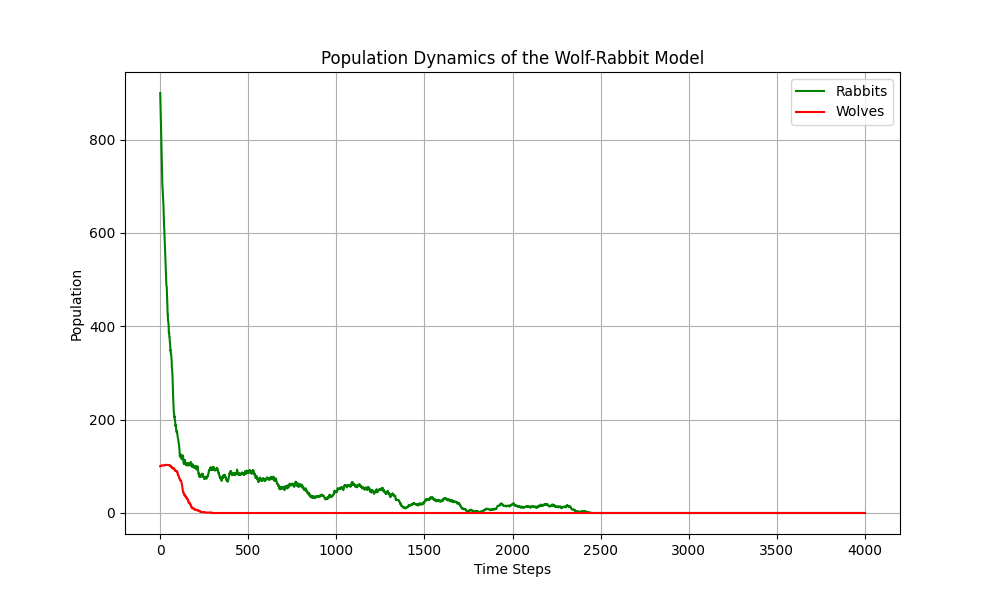
\includegraphics[width=\textwidth]{media/population_dynamics_ex02.png}
\caption{
    \textbf{Population Dynamics}
	$t_d^r = 50$
    }
\label{fig:ex02}
\end{figure}

